\documentclass[./Main.tex]{subfiles}
\graphicspath{{./Fig/}}
\begin{document}

%% tikzデモ
\chapter{模式図の例}
tikzというライブラリを使うと,コマンドをTeXのソースファイルに記述することで,図が書けます。
以下の図がその例。一部,GPTで生成したものもあるので,若干変です。

\begin{tikzpicture}[font = \sansmath]
  \coordinate (O) at (0,0);

  % ball background color
  \shade[ball color = blue, opacity = 0.2] (0,0) circle [radius = 2cm];

  % cone
  \begin{scope}
    \def\rx{0.71}% horizontal radius of the ellipse
    \def\ry{0.15}% vertical radius of the ellipse
    \def\z{0.725}% distance from center of ellipse to origin

    \path [name path = ellipse]    (0,\z) ellipse ({\rx} and {\ry});
    \path [name path = horizontal] (-\rx,\z-\ry*\ry/\z)
                                -- (\rx,\z-\ry*\ry/\z);
    \path [name intersections = {of = ellipse and horizontal}];

    % radius to base of cone in ball
    \draw[fill = gray!50, gray!50] (intersection-1) -- (0,0)
      -- (intersection-2) -- cycle;
    % base of cone in ball
    \draw[fill = gray!30, densely dashed] (0,\z) ellipse ({\rx} and {\ry});
  \end{scope}

  % label of cone
  \draw (0.25,0.4) -- (0.9,0.1) node at (1.05,0.0) {$q$};

  % ball
  \draw (O) circle [radius=2cm];
  % label of ball center point
  \filldraw (O) circle (1pt) node[below] {$P$};

  % radius
  \draw[densely dashed] (O) to [edge label = $r$] (-1.33,1.33);
  \draw[densely dashed] (O) -- (1.33,1.33);

  % cut of ball surface
  \draw[red] (-1.35,1.47) arc [start angle = 140, end angle = 40,
    x radius = 17.6mm, y radius = 14.75mm];
  \draw[red, densely dashed] (-1.36,1.46) arc [start angle = 170, end angle = 10,
    x radius = 13.8mm, y radius = 3.6mm];
  \draw[red] (-1.29,1.52) arc [start angle=-200, end angle = 20,
    x radius = 13.75mm, y radius = 3.15mm];

  % label of cut of ball surface
  \draw (-1.2,2.2) -- (-0.53,1.83) node at (-1.37,2.37) {$A$};
\end{tikzpicture}


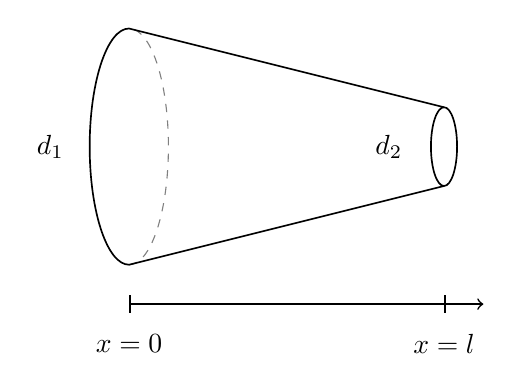
\begin{tikzpicture}
	\draw[dashed,color=gray] (0,0) arc (-90:90:0.5 and 1.5);% right half of the left ellipse
	\draw[semithick] (0,0) -- (4,1);% bottom line
	\draw[semithick] (0,3) -- (4,2);% top line
	\draw[semithick] (0,0) arc (270:90:0.5 and 1.5);% left half of the left ellipse
	\draw[semithick] (4,1.5) ellipse (0.166 and 0.5);% right ellipse
	\draw (-1,1.5) node {$\varnothing d_1$};
	\draw (3.3,1.5) node {$\varnothing d_2$};
	\draw[|-,semithick] (0,-0.5) -- (4,-0.5);
	\draw[|->,semithick] (4,-0.5) -- (4.5,-0.5);
	\draw (0,-1) node {$x=0$};
	\draw (4,-1) node {$x=l$};
\end{tikzpicture}


% 視点設定
\tdplotsetmaincoords{65}{120}

\begin{tikzpicture}[tdplot_main_coords, scale=3]

\def\R{1.2}

%========================
% 球本体(外周円)
%========================
\shade[ball color=gray!20, opacity=0.6] (0,0,0) circle (\R);

%========================
% 赤道(実線+破線)
%========================
\tdplotdrawarc[thick]{(0,0,0)}{\R}{0}{180}{}{}
\tdplotdrawarc[dashed]{(0,0,0)}{\R}{180}{360}{}{}

%========================
% 経線(縦の円)
%========================
\tdplotsetrotatedcoords{90}{0}{0}
\tdplotdrawarc[thick]{(0,0,0)}{\R}{0}{180}{}{}
\tdplotdrawarc[dashed]{(0,0,0)}{\R}{180}{360}{}

%========================
% 別の経線
%========================
\tdplotsetrotatedcoords{90}{60}{0}
\tdplotdrawarc[thick]{(0,0,0)}{\R}{0}{180}{}{}
\tdplotdrawarc[dashed]{(0,0,0)}{\R}{180}{360}{}

%========================
% 極
%========================
\node at (0,0,\R+0.15) {N};
\node at (0,0,-\R-0.15) {S};

\end{tikzpicture}

%%%%%%%%%%%%%%%%%%%%%%%%%%%%%%%%%%%%%
\begin{tikzpicture}[scale=1.2, >=stealth]

% パラメータ
\def\v{3}        % 初速度ベクトル長
\def\ang{45}     % 発射角
\def\g{0.5}      % 重力係数(見た目調整)

%========================
% 座標軸
%========================
\draw[->] (-0.5,0) -- (6,0) node[right] {$x$};
\draw[->] (0,-0.5) -- (0,4) node[above] {$y$};

%========================
% 放物線軌道 y = x tanθ - g x^2
%========================
\draw[thick, domain=0:5, smooth, variable=\x]
    plot ({\x}, {\x*tan(\ang) - \g*\x*\x});

%========================
% 初速度ベクトル
%========================
\draw[->, thick] (0,0) -- ({\v*cos(\ang)}, {\v*sin(\ang)})
    node[midway, above right] {$\vec{v}_0$};

%========================
% 角度表示
%========================
%\draw pic["$\theta$", draw=black, angle radius=12mm]
%    {angle = (1,0)--(0,0)--({cos(\ang)},{sin(\ang)})};

%========================
% 重力ベクトル
%========================
\draw[->, thick] (4.5,3.5) -- (4.5,2.8) node[right] {$\vec{g}$};

%========================
% 初期点
%========================
\fill (0,0) circle (1.5pt);

\end{tikzpicture}
%%%%%%%%%%%%%%%%%%%%%%%%%%%%%%%%%%%%%%

\ifSubfilesClassLoaded{
\printbibliography[title=参考文献]
}{}

\end{document}